\chapter{Task 4 --- Controlled Learning-Rate Experiment}
\label{ch:task4}

%-------------------------------------------------------

Task 4 asks me to choose one factor, compare the baseline with at least
one alternative under otherwise fixed settings, train each for 10
epochs, compare their curves, and explain which configuration I would
select and why. Section \ref{sec:experiment-design} describes the
setup and Section \ref{sec:task4} the results and the selection.

%%%%%%%%%%%%%%%%%%%%%%%%%%%%%%%%%%%%%%%%%%%%%%%%%%%%%
\section{Experiment Design}
\label{sec:experiment-design}
%%%%%%%%%%%%%%%%%%%%%%%%%%%%%%%%%%%%%%%%%%%%%%%%%%%%%

The factor I chose to study is the learning rate. Besides the baseline
($\eta = 0.01$), I trained two alternatives, one ten times smaller
($\eta = 0.001$) and one ten times larger ($\eta = 0.1$). Everything else
is identical to Table \ref{table:config}: same optimizer and momentum,
same batch size, same split, same seed, same initial weights and same
batch order. The three configurations are listed at the top of
\texttt{main.py} (Listing \ref{lst:configs}).

\lstinputlisting[language=Python, firstline=30, lastline=39,
    firstnumber=auto,
    caption={The three configurations (\texttt{main.py}).},
    label={lst:configs}]{../main.py}

\textbf{Selection rule.} The rule was fixed before looking at any
results: the configuration with the highest validation accuracy after
epoch 10 is selected, with lower validation loss as the tie-breaker. The
test set is only loaded after this choice is made, and only once.


%%%%%%%%%%%%%%%%%%%%%%%%%%%%%%%%%%%%%%%%%%%%%%%%%%%%%
\section{Results and Selection}
\label{sec:task4}
%%%%%%%%%%%%%%%%%%%%%%%%%%%%%%%%%%%%%%%%%%%%%%%%%%%%%

Figure \ref{fig:compare} shows the
training and validation curves side by side, Figure
\ref{fig:compare-epoch1} compares the first epoch, Figure
\ref{fig:compare-val} zooms in on validation accuracy, and Table
\ref{table:compare} summarizes the results.

\begin{figure}[H]
    \centering
    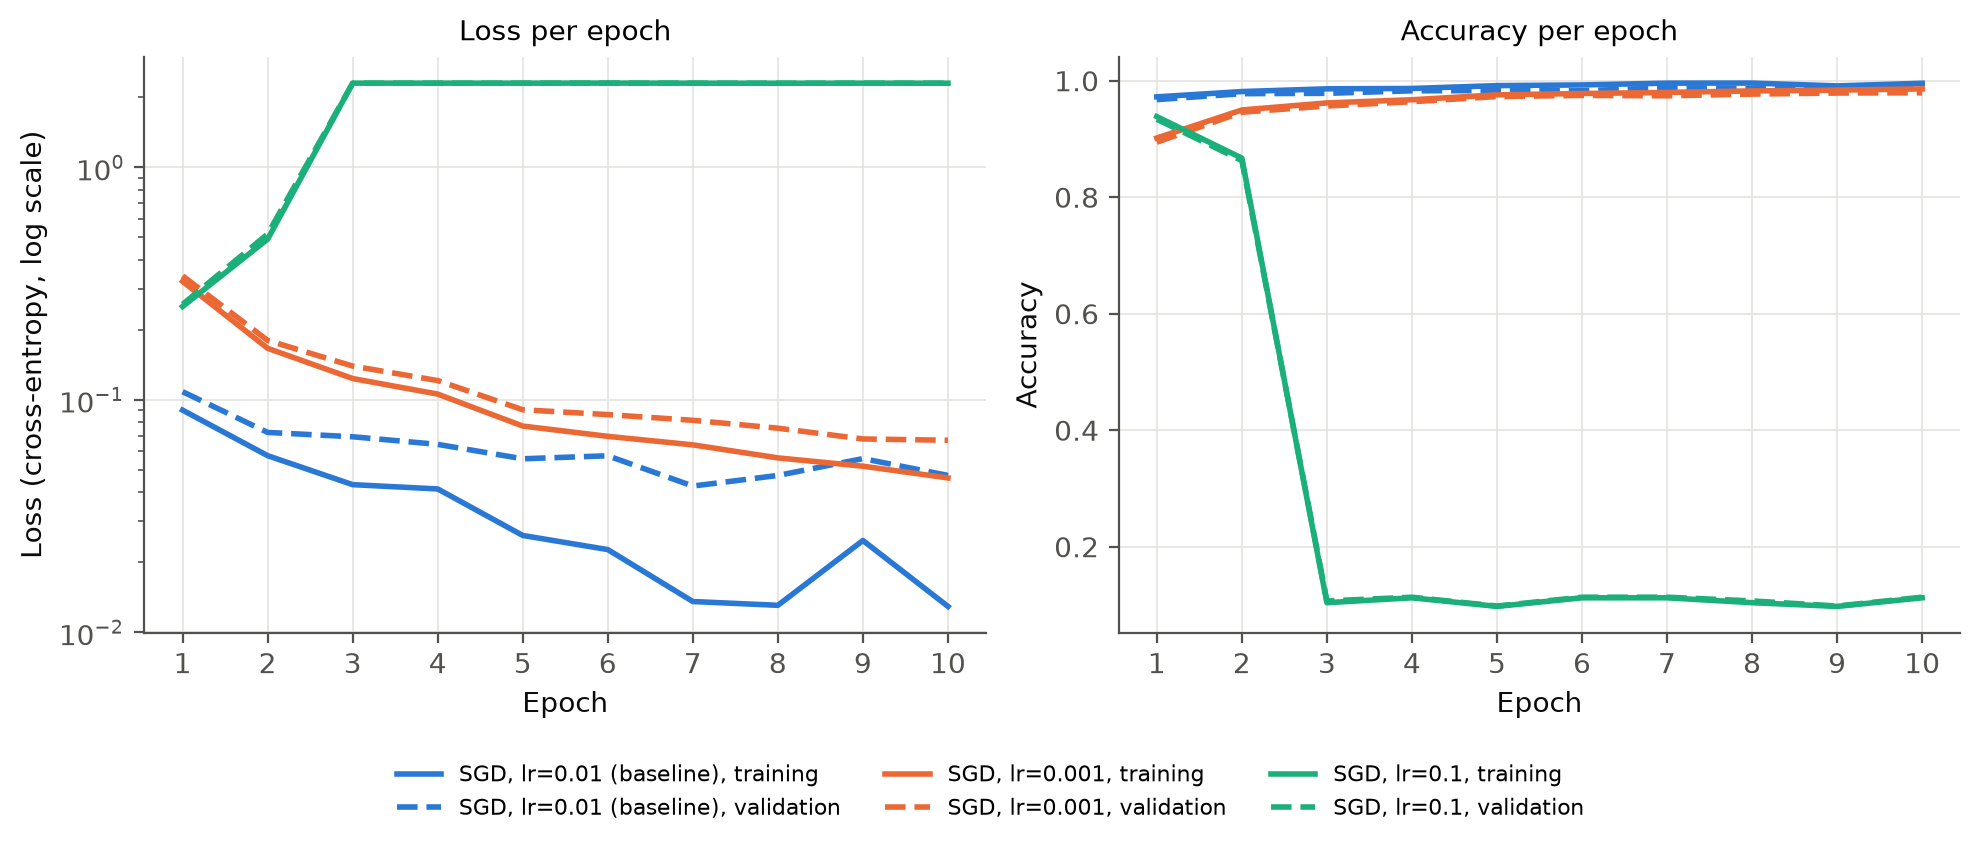
\includegraphics[width = \textwidth]{compare_curves.png}
    \caption[Learning-rate comparison: loss and accuracy curves.]%
    {Training (solid) and validation (dashed) loss and accuracy per epoch
    for the three learning rates (SGD, momentum 0.9, batch size 64). The
    loss axis is logarithmic.}
    \label{fig:compare}
\end{figure}

\begin{figure}[H]
    \centering
    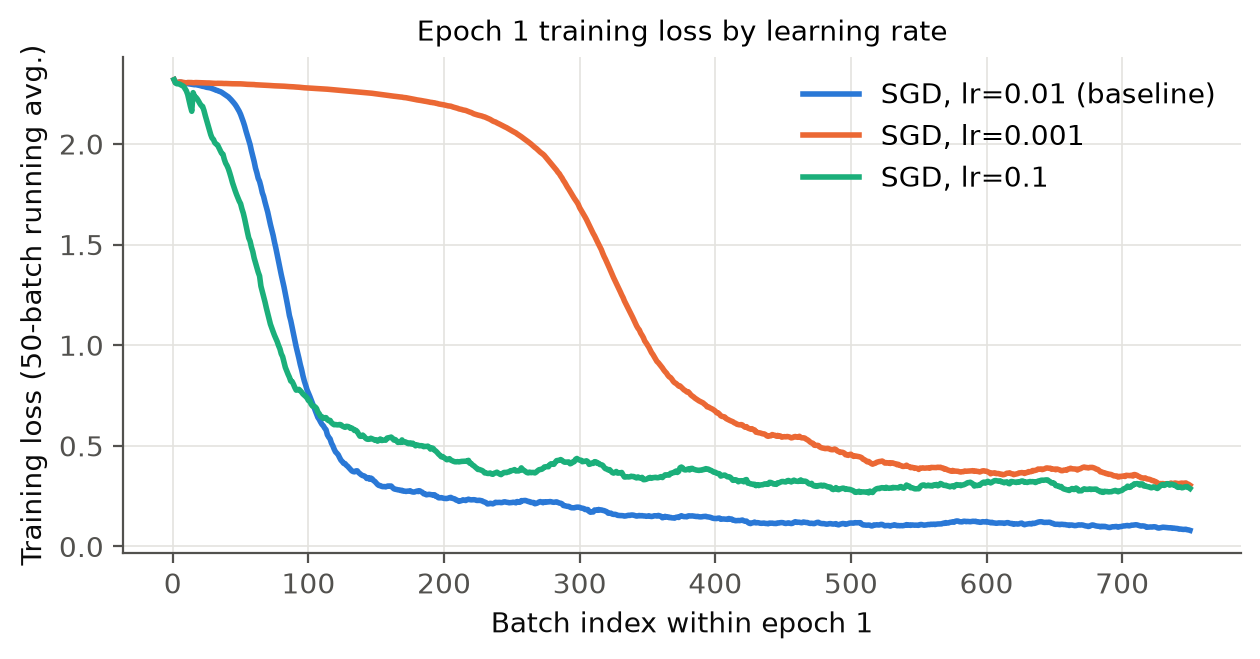
\includegraphics[width = 0.88\textwidth]{compare_epoch1_loss.png}
    \caption[Learning-rate comparison: first-epoch loss.]%
    {Training loss (50-batch running average) during the first epoch for
    the three learning rates.}
    \label{fig:compare-epoch1}
\end{figure}

\begin{figure}[H]
    \centering
    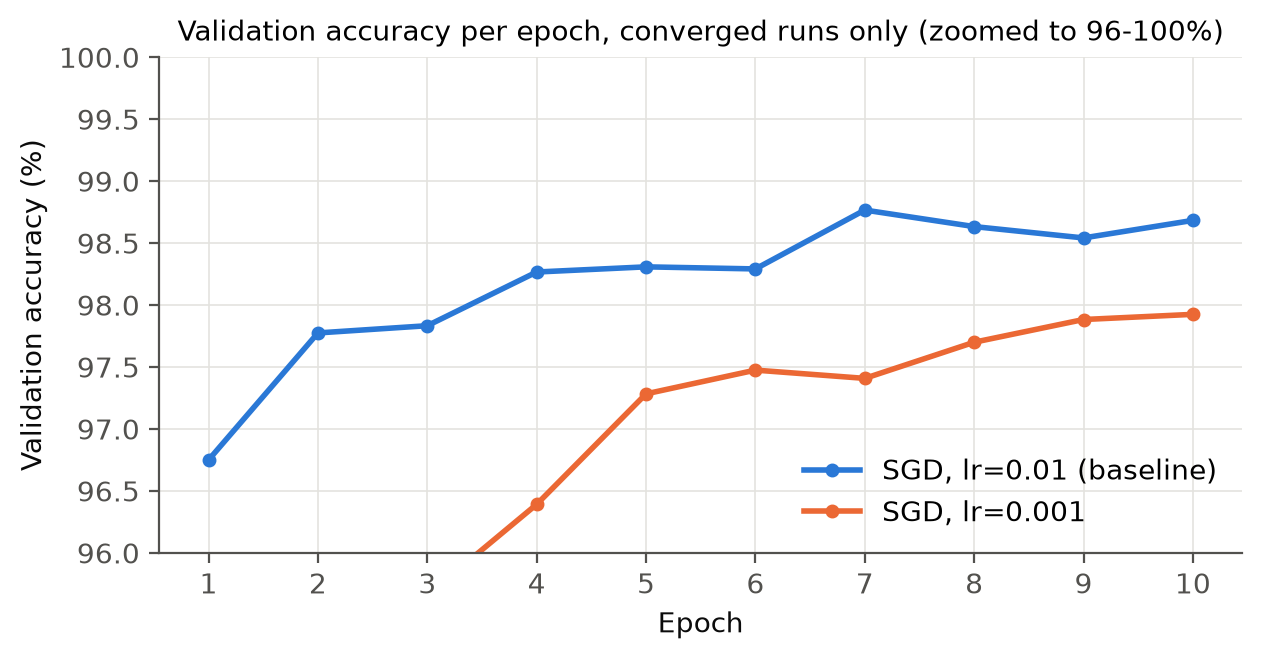
\includegraphics[width = 0.88\textwidth]{compare_val_acc.png}
    \caption[Learning-rate comparison: validation accuracy (zoom).]%
    {Validation accuracy per epoch for $\eta = 0.01$ and $\eta = 0.001$,
    zoomed to 96--100\%. The $\eta = 0.1$ run is left out because it stays
    near 11\% after epoch 3.}
    \label{fig:compare-val}
\end{figure}

\begin{table}[h]
    \centering
    \caption[Learning-rate comparison summary.]%
    {Learning-rate comparison. Final values are after epoch 10; the gap
    is training accuracy minus validation accuracy at epoch 10.}

    \begin{tabular}{l|c|c|c}
        \specialrule{1.5pt}{0pt}{0pt}
        & $\eta = 0.001$ & $\eta = 0.01$ (baseline) & $\eta = 0.1$ \\
        \hline\hline
        Val.\ accuracy after epoch 1 & 89.44\% & 96.75\% & 93.38\% \\
        \specialrule{0.5pt}{0pt}{0pt}
        Batch where running acc.\ passes 90\% & 714 & 151 & 228 \\
        \specialrule{0.5pt}{0pt}{0pt}
        Final training accuracy & 98.60\% & 99.56\% & 11.22\% \\
        \specialrule{0.5pt}{0pt}{0pt}
        Final validation accuracy & 97.92\% & \textbf{98.68\%} & 11.33\% \\
        \specialrule{0.5pt}{0pt}{0pt}
        Final validation macro-F1 & 0.9790 & \textbf{0.9867} & 0.0203 \\
        \specialrule{0.5pt}{0pt}{0pt}
        Final validation loss & 0.0670 & \textbf{0.0473} & 2.3030 \\
        \specialrule{0.5pt}{0pt}{0pt}
        Best validation accuracy (epoch) & 97.92\% (10) & 98.77\% (7) & 93.38\% (1) \\
        \specialrule{0.5pt}{0pt}{0pt}
        Train--val.\ accuracy gap & 0.67 pts & 0.88 pts & --- \\
        \specialrule{1.5pt}{0pt}{0pt}
    \end{tabular}
    \label{table:compare}
\end{table}

\textbf{Small learning rate ($\eta = 0.001$): too slow.} With steps ten
times smaller, the network stays on the initial plateau much longer. In
the first epoch the loss is still 2.19 after 200 batches, and the running
accuracy passes 90\% only at batch 714, almost five times later than the
baseline (Figure \ref{fig:compare-epoch1}). After one epoch it has 89.4\%
validation accuracy, against 96.8\% for the baseline. It keeps
improving steadily and never shows instability, but after 10 epochs it
reaches only 97.92\%, about where the baseline was after epoch 3. Its
validation loss is still going down at epoch 10, so this run has not
converged yet: it is slightly \emph{underfitting} within the 10-epoch
budget. Its train--validation gap is the smallest (0.67 points), but
only because it has not fit the training data as tightly yet.

\textbf{Large learning rate ($\eta = 0.1$): fast, then unstable.} At first
the large steps help: in Figure \ref{fig:compare-epoch1} its loss falls
earlier than the baseline's. But the curve is noisier, with a loss spike
to 3.55 at batch 15, and in the second half of the epoch its loss stays
higher (0.30 on average, against 0.11 for the baseline), because the steps are too big
to settle into a good minimum. After epoch 1 its validation accuracy is
93.4\%. In epoch 2 it gets worse (86.3\%), and in epoch 3 training
collapses. From then on the loss stays at 2.303, which is exactly
$\ln 10$, and accuracy stays at about 11\%: the network has collapsed to
predicting the same digit for every image, which is why its validation
macro-F1 is only 0.0203. Training and validation accuracy are equally
bad, which points to a failure of the optimization itself.

\textbf{Selection.} Following the rule set in Section
\ref{sec:experiment-design}, the selected configuration is the
\textbf{baseline, $\eta = 0.01$}. It has the highest final validation
accuracy (98.68\%), the highest validation macro-F1 (0.9867) and the
lowest validation loss (0.0473). It also converges much faster than
$\eta = 0.001$ and is stable, while $\eta = 0.1$ diverges. Its
generalization gap (0.88 points) is a little larger than that of
$\eta = 0.001$, but its validation accuracy is still 0.76 points higher.
With more epochs $\eta = 0.001$ might catch up. Within the 10 epochs
required here, 0.01 is the better choice.
